\documentclass[11pt]{article}

\usepackage[final]{acl}
\usepackage{times}
\usepackage{latexsym}
\usepackage[T1]{fontenc}
\usepackage[utf8]{inputenc}
\usepackage{microtype}
\usepackage{inconsolata}
\usepackage{graphicx}
\usepackage{amsmath}

\title{Where Do Multilingual Encoders Compute Hindi Grammar?}

\author{Ekansh Goyal \and Varun Gupta \\
  International Institute of Information Technology, Hyderabad}

\begin{document}
\maketitle

\section{Data and Methods}
\label{sec:methods}

\paragraph{Tasks and data.}
Both tasks use news sentences from the Hindi-Urdu Treebank \citep{bhatt2009}.
For word order, each of 8,923 written sentences is paired with one grammatical reordering of its own words.
The model should prefer the written one.
For agreement, we take 459 past-tense transitive clauses whose \emph{ne}-marked subject and bare object differ in gender or number.
Each clause appears in its attested order and in up to 30 reorderings, 5,265 orders in all.
The verb agrees with the bare object \citep{mohanan1994}, so every order has a correct verb form and a wrong one that agrees with the subject (Figure~\ref{fig:design}).

\paragraph{Models.}
We study MuRIL \citep{khanuja2021} and XLM-R-large \citep{conneau2020}.
MuRIL has 12 layers and 144 heads and is trained on Indian languages and English.
XLM-R-large has 24 layers and 384 heads and is trained on 100 languages.
They differ in training data and depth, so a finding in both is unlikely to be an accident of one model.

\paragraph{Scoring.}
Both are masked encoders, so we score a sentence word by word.
The subtokens of a word are masked from left to right, and each is scored given the rest of the sentence \citep{kauf2023}.
This pseudo-log-likelihood is not true surprisal, and we report it in bits.
For word order, the metric of a run is minus its mean per-word surprisal.
For agreement, it is the margin $M=\log_2 P(\text{correct})-\log_2 P(\text{wrong})$ of the two verb forms.

\paragraph{Patching.}
The \emph{clean run} is the sentence as written.
The \emph{corrupted run} is its reordering for word order, and for agreement the sentence with the whole object phrase masked.
The \emph{gap} is the clean metric minus the corrupted metric.
Patching copies one component's output, an attention head or an MLP, from the clean into the corrupted run.
We read the share of the gap it restores.
We screen all components with attribution patching \citep{syed2024}, confirm them by exact patching, and trace paths with path patching \citep{wang2023}.
The corruption decides which components are found \citep{zhang2024}: masking finds those that carry the object's features to the verb.
Masking is a training operation of these encoders, but not usually on a whole phrase, so Section~\ref{sec:swap} retests the findings on whole sentences.

\paragraph{Ablation.}
We ablate a component by replacing its output with its mean over 300 held-out sentences, with separate means for special, masked and other positions.
Zero ablation serves as a check.
Every ablation must keep held-out surprisal within 2 nats per subtoken of the unablated model.

\paragraph{Evaluation.}
\emph{Faithfulness} is the share of the gap restored by patching only a set of components, and \emph{necessity} is the share lost when the set is ablated.
Both are ratios of sums over items with a gap above 0.05 bits, so they can exceed one.
We choose the top ten heads and the top five MLPs on a \emph{selection half} of the documents and measure them once on a \emph{held-out half} (Appendix~\ref{app:data}).
Heads are compared with 100 random head sets, each head swapped for another in its block.
A model has one MLP per block, too few to match, so MLPs are judged separately (Section~\ref{sec:redundancy}).
Intervals are 95\% bootstrap intervals over documents (2,000 resamples) and are descriptive.
Tests flip the signs of whole documents in 10,000 permutations, so the smallest $p$ is $10^{-4}$.
Tests of what the components read use documents in neither half.

\begin{figure*}[t]
  \centering
  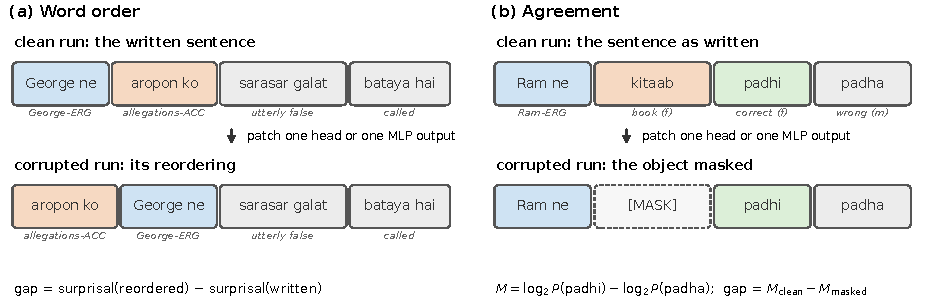
\includegraphics[width=\textwidth]{figures/fig1_design.pdf}
  \caption{The two tasks. In each panel the clean run (top) is the sentence as written, and the corrupted run (bottom) is its reordering (a) or the sentence with the object masked (b). Patching copies one component's output from the clean into the corrupted run. The agreement sentence is constructed. ERG: ergative; f, m: feminine, masculine.}
  \label{fig:design}
\end{figure*}

\bibliography{custom}

\end{document}
